\chapter{The SpinTaylorF2 waveform model} 

\label{chap:SpinTaylorF2} 
The SpinTaylorF2 waveform~\cite{Lundgren2014} is a single spin, frequency domain
waveform that incorporates the effects of precession.  The waveform model
assumes one component of the binary to have negligible or zero spin, and
describes the inspiral phase~\cite{Event_0} of the signal. We will therefore
restrict our attention to NS-BH binaries since the neutron star in these systems
are expected to have neglible spins. 

Consider a NS-BH binary, with black hole
mass $m_{1}$ and dimensionless spin $\chi_{1} = |\mathbf{S}|/m_{1}^2$ where
$|\mathbf{S}|$ is the spin angular momentum of the black hole, and a neutron
star with mass $m_{2}$ and zero spin. The the symmetric mass ratio $\eta$ is
defined as $\eta=m_{1}m_{2}/M^2$. where $M$ corresponds to the total mass of the
binary $(m_{1} + m_{2})$.  Further, we can define the total angular momentum
vector $\mathbf{J}=\mathbf{L} + \mathbf{S}$ of the binary as a sum of the
orbital anuglar momentum vector $\mathbf{L}$. We also define a quantity
$\kappa=\hat{\mathbf{L}}\cdot\hat{\mathbf{S}}$, to describe the alignment of the
$\mathbf{L}$ and $\mathbf{S}$: $\kappa=0$ corresponds to the situation where
$\mathbf{L}$ and $\mathbf{S}$ are perpendicular to each other, and $\kappa=\pm
1$ correponds to the aligned (anti-aligned) case. In addition, polar angles
$(\theta_{J}, \psi_{J})$  describes the relative orientation  of the total
angular momentum vector $\mathbf{J}$ with the line of sight unit vector
$\hat{\mathbf{N}}$ (see, for eg.,~\cite{thetaJ} for a graphical representation
of the coordinates used). All the equations in the report are written in 
$\left[G = c = M_{\odot }= 1\right]$ units.

\section{Coordinate systems}
If the black hole has non-zero spin, and the spin-angular momentum $\mathbf{S}$
is  not aligned with the orbital orbital angular momentum $\mathbf{L}$ of the
binary, the plane of orbital motion inclines and precesses over
time~\cite{Apostolatos1994}: both $\mathbf{L}$ and $\mathbf{S}$  would precess
about the total angular momentum vector $\mathbf{J}$ (see Eq.~(11)
in~\cite{Apostolatos1994} for evolution equations of $\mathbf{L}$ and
$\mathbf{S}$). Further, if $\mathbf{L}$ and $\mathbf{S}$ do not cancel each
other (i.e. are not antialigned and almost equal in magnitude)  the binary
undergoes simple precession~\cite{Apostolatos1994}, where $\mathbf{J}$ remains
nearly fixed during the inspiral, and $\mathbf{L}$ and $\mathbf{S}$ precesses
about $\mathbf{J}$ with a uniform angular velocity. The SpinTaylorF2 waveform
assumes simple precession~\cite{Lundgren2014}, and breaks down  when the
assumption is no longer applicable.
\label{fig:waveforms} 
\begin{figure}[t]
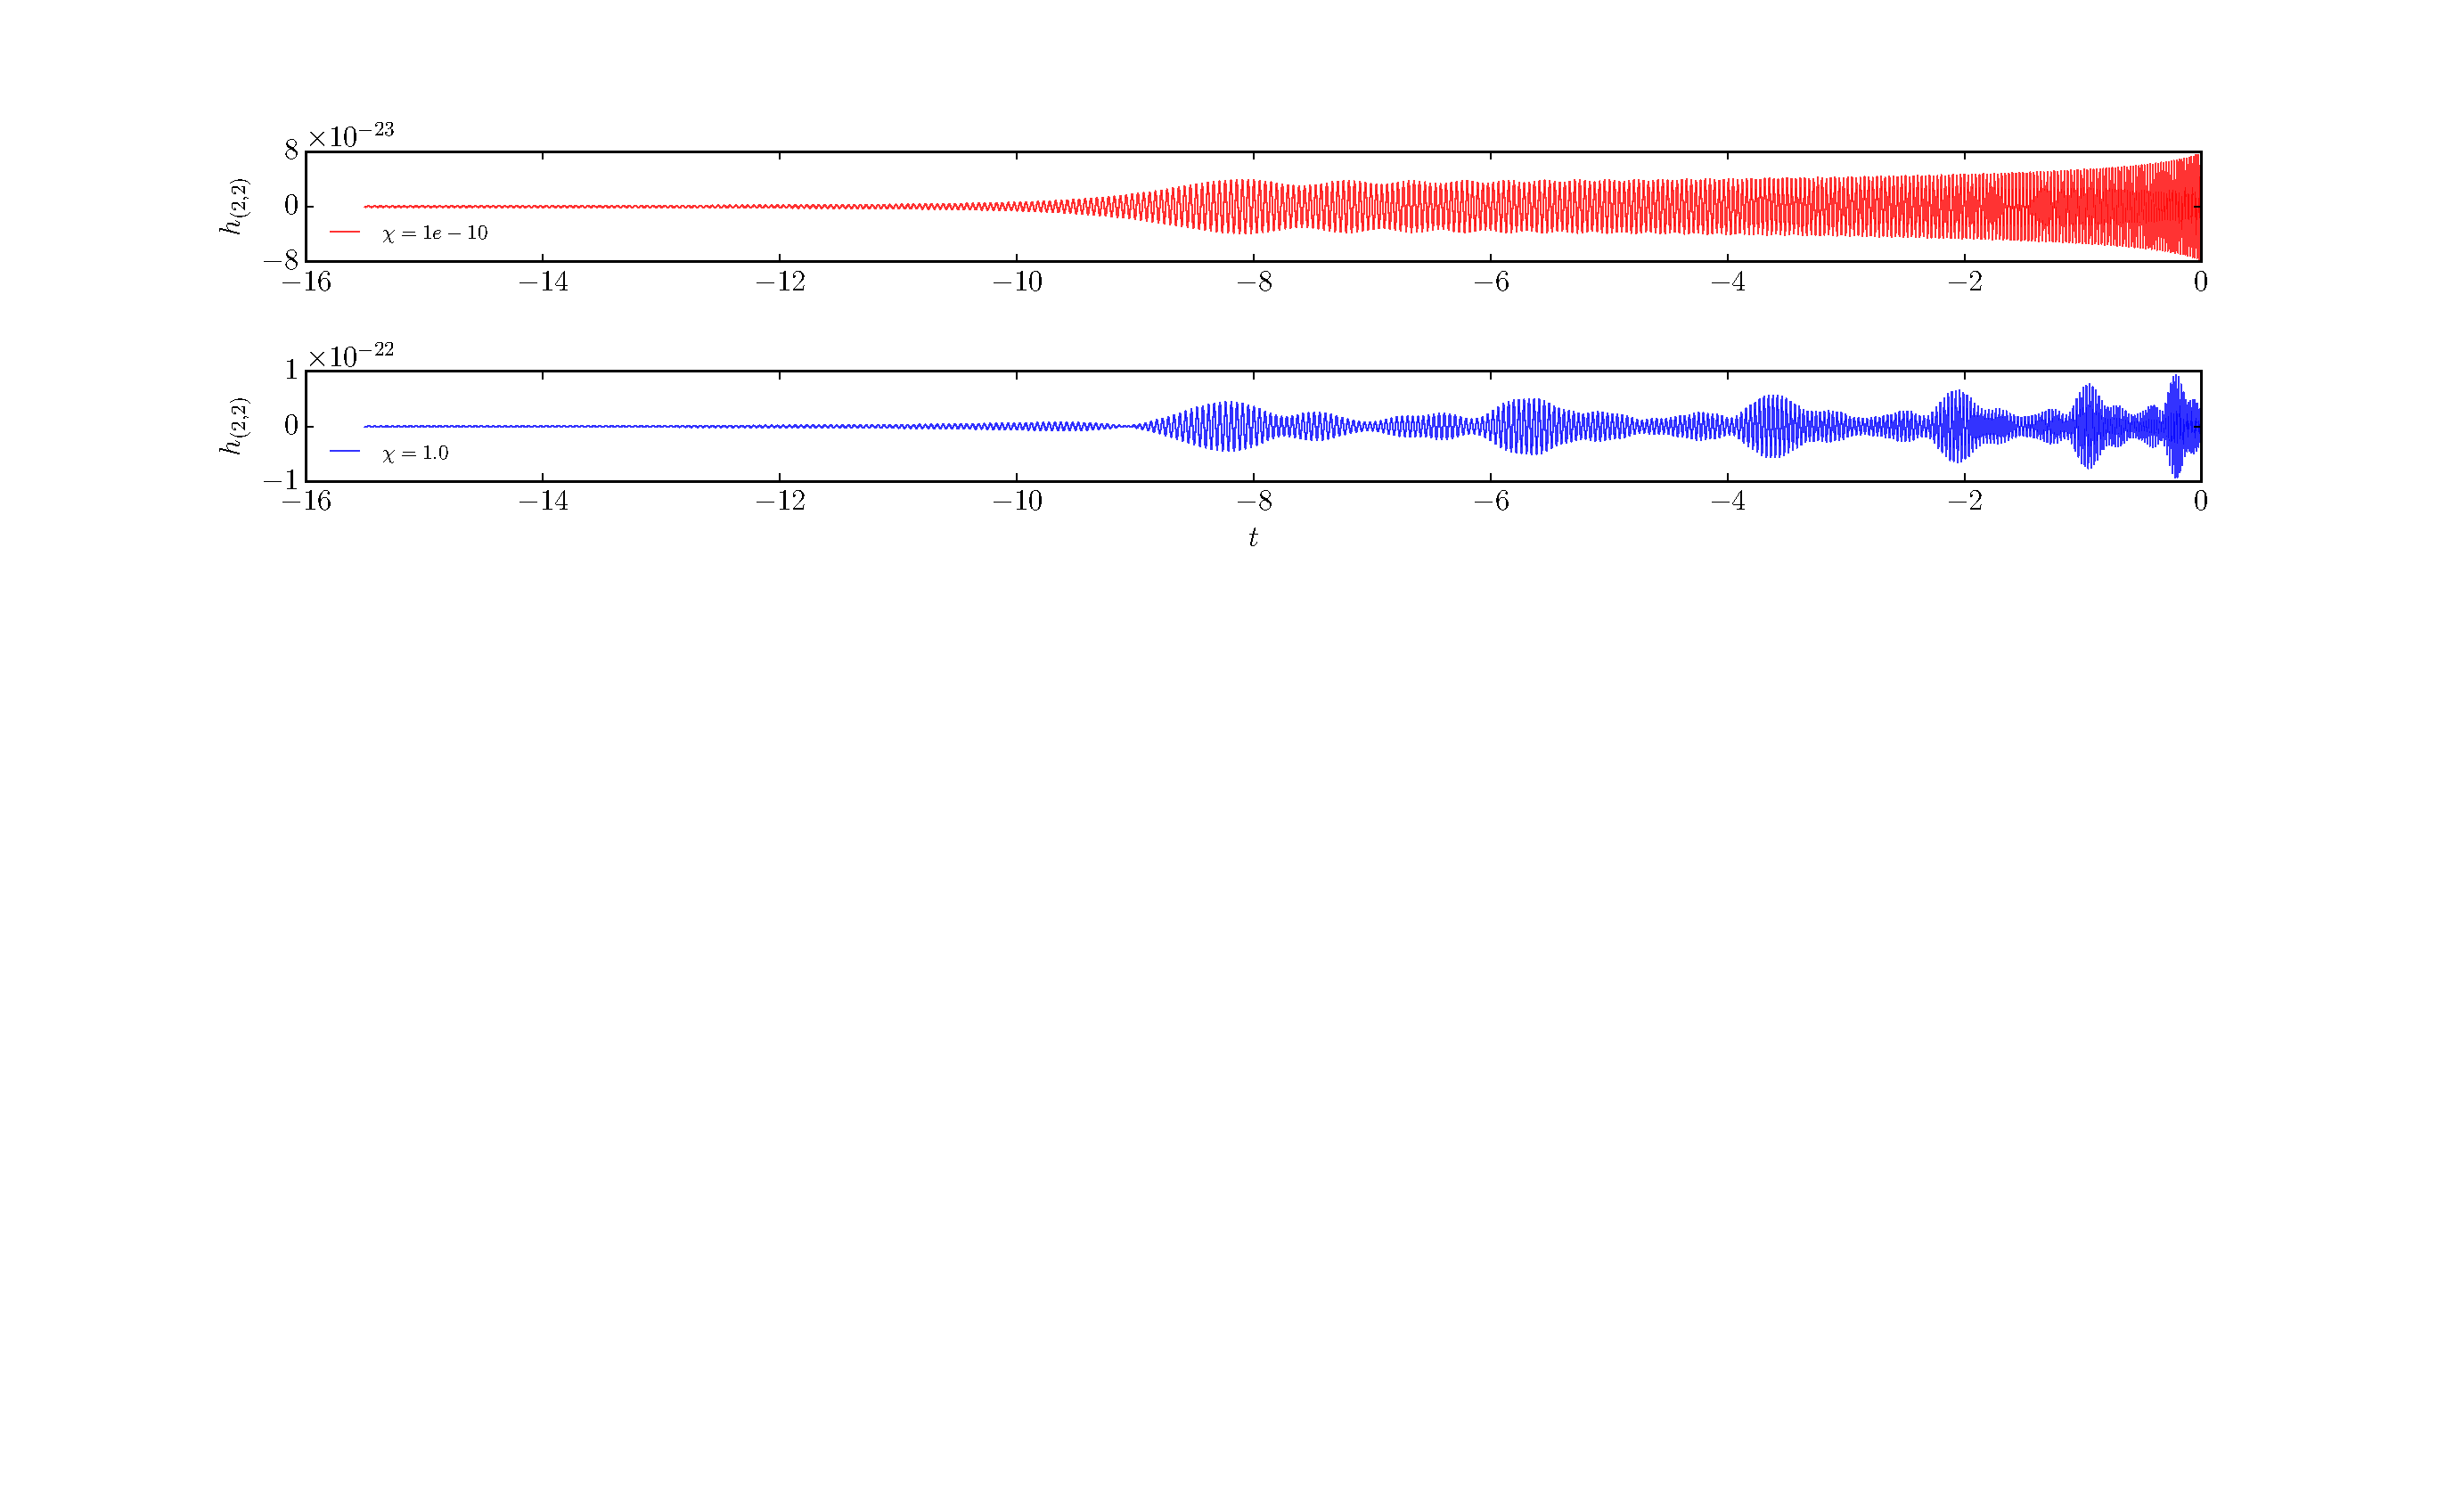
\includegraphics[width=\textwidth]{./images/TD_waveforms_comparison.pdf}
\caption{SpinTaylorF2 waveforms for non-precessing (red) and precessing (blue) system. 
The modulations in the waveform amplitude due to precession is clearly visible in the 
bottom figure.} 
\centering 
\end{figure}

\section{The construction of SpinTaylorF2}

The precession of the orbital plane leads to modulations in the gravitational
wave amplitude and phase in the observer's frame of reference (see Fig.~\ref{fig:waveforms}).
However, the precessing waveform in the observer's frame can be decomposed into
non-precessing waveform acted upon by a time-dependent rotation~\cite{Boyle2011,
Rotation}. The time-dependent rotation relates the observer's frame of reference
aligned with $\mathbf{J}$ to a frame that co-rotates with the precession of the
orbital angular momentum vector $\mathbf{L}$. The precessing waveform can then
be expressed as a weighted sum of the co-rotating frame amplitudes
$\tilde{h}^{l,m}$ (see Eq. (3) in~\cite{Lundgren2014}):
\begin{equation}   
h_{+} + i h_{\times} = e^{-2 \psi}
\sum_{l,m,m^{\prime}} \mathcal{D}^{l}_{m^{\prime},m} \left(\alpha, \beta, \gamma\right)
\tilde{h}^{l,m}(t){}_{-2}Y_{l,m^{\prime}}\left(\theta,\phi\right)e^{-i m \Phi},
\end{equation}   
where $\mathcal{D}^{l}_{m^{\prime},m}$ is the Wigner rotation matrix of
SU2~\cite{Boyle2011}, and $(\alpha, \beta, \gamma)$ are the time- dependent
Euler angles that relate the co-rotating frame to the observer's frame of
reference. See~\cite{Lundgren2014} for complete definitions. Considering only
the leading order $(l=2, |m| = 2)$ mode, we can express the above expression in
frequency domain using the stationary phase approximation~\cite{Lundgren2014,
Creighton}.  Upon simplification, one arrives at the following expression for
the SpinTaylorF2 waveform (see Eq. (12--13) in~\cite{Lundgren2014}):
\begin{equation}  
\label{STF2_main} 
h_{+}(f) =
\dfrac{2\pi M_{c}^{2}}{D}\sqrt{\dfrac{5}{96\pi}}(\pi M
f)^{-7/6}\sum_{m}z_{m}e^{i(\Psi - 2\zeta) + i m \alpha},
\end{equation} 
where $D$ corresponds to the distance to the source, and $M_{c}$ corresponds to
chirp mass~\cite{Creighton} of the binary. The expressions for $z_{m}, \alpha,
\Psi$ and $\zeta$  can be found in~\cite{Lundgren2014}, we omit them for
brevity. Fig.~(\ref{fig:waveforms}), shows  time-domain plot of the full
SpinTaylorF2 waveform for a precessing and non-precessing case. Each term in the
summation in Eq.~(\ref{STF2_main}) represents a single sideband that is
modulated in amplitude and phase depending on the value of $m$.  We observed
that in  the non-precessing case, only the $m=2$ sideband has a non-zero
amplitude; however, for a precessing system, all the sidebands develop a non-
zero amplitude. Thus, we would expect that the single to noise ratio (SNR) from
the total waveform would be sub-divided into the SNR contribution from each of
the individual sidebands in case of precession systems. In the following section, 
we discuss how the SNR of the total waveform is distributed among the sidebands
by computing overlap between the particular sideband and the full waveform.






